\section{Pipeline}
\begin{table}[t]
  \resizebox{\linewidth}{!}{
  \begin{tabular}{l|p{8cm}}
    \textbf{symbol} & \textbf{stands for}\\
     $X$    & Georeferenced image set \\
     $I_i$    & Georeferenced image \\
     $Y$    & Annotations classes for $X$\\
     $y_i$    & Annotation class in $Y$\\
     $\hat{I_j}$ & Template image\\
     $I'$ & Target Image\\
     & \\
     \textbf{term} & \textbf{stands for}\\
     \textit{Template Image} $\hat{I_j}$    & A synthetic transformation of input image $I$ towards the class $y_j$ \\
     \textit{Target Image} $I'$    & The natural image which is most visually similar to the template image \\
    \textit{ Data Clustering}    & A process which groups images in $X$ according to visual similarity (e.g urban vs rural)\\
     \textit{Data Augmentation}    & A process which looks for images taken in the surrounding areas of the georeferenced images in $X$\\
     \textit{Classifier}   & A deep-learning framework that is able to classify images into one of the classes in $Y$\\
     \textit{Generator} $(GAN)$    & A deep-learning based generative framework to produce images similar to the ones in  $X$\\
     $DGN-AM$    & A framework that, given the GAN and the Classifier, transforms an input image into the template image.\\
            \end{tabular}}
  \caption{Notations and Terms.}\label{notations}
\end{table}
With the motivation of creating a streamlined framework, we propose an end-to-end pipeline for explaining urban image categories, which is illustrated in Figure \ref{fig:pipeline}.% This pipeline makes it easier for the reader to understand and infer the incremental processes involved in explaining a model. 
%The goal of this pipeline is to articulate a framework under which anyone with an arbitrarily set of annotated image data $ X = { I_1, I_2 ... . I_n  }$ annotated in classes $Y = {y_1 , y_2 , ... ,y_k}$, can transform natural images between classes. What this entails is that the process should be able to transform an arbitrary image $I_i$ belonging to class $y_i \in Y$ , to image $I_j$ from class $y_j \in Y$.  Doing so, would allow us to visually reason about the discriminative properties between classes $y_i , y_j \in Y$. We could visually understand what are the salient characteristics learned by a classifier network, that makes it to classify images into the respective classes $y_i,y_j$. These questions might be trivial for tangible classes of objects, but are still a mystery for intangible classes representing concepts like affects and aesthetics.
The system allows anyone with an arbitrarily set of  image data $ X = { I_1, I_2 ... . I_n  }$ annotated in classes $Y = {y_1 , y_2 , ... ,y_k}$, to transform natural images between classes: the pipeline can transform an arbitrary image $I_i$ belonging to class $y_i \in Y$ , to image $I_j$ from class $y_j \in Y$.  This allows  to visually reason about the discriminative properties between classes $y_i , y_j \in Y$, and visually understand what are the salient characteristics %learned by a classifier network, 
that drive a classifier to distinguish between  classes $y_i,y_j$. These questions might be trivial for tangible classes of objects, but still remain largely unexplored for intangible classes representing concepts like affects and aesthetics.
\par 
%Similar to how designers make prototype models of objects before actually committing to the production, t
This pipeline approaches the transformation problem in two phases. Assuming the previous example where we transform images from class $y_i$ to class $y_j$, the first step is to produce a prototype image or a template image $\hat{I_j}$, that represents the basic traits of the %an intermediate step between the original and transformed image and that represents 
the destination class $y_j \in Y$. The second step is to 
%"Productize" so to speak 
match this template image $\hat{I_j}$, 
with the closest natural image in $X$.
%which implies getting as close as possible to this template in the natural image space.
 In mathematical terms, we want to choose a target image $I'$ from $X$ so as to minimize $E(I' , \hat{I_j} )$ , where $E(I_1, I_2)$ is some error measure that quantifies visual error between two images. This image $I'$ is effectively a natural transformed image.
 \begin{figure*}[ht]
	\centering
	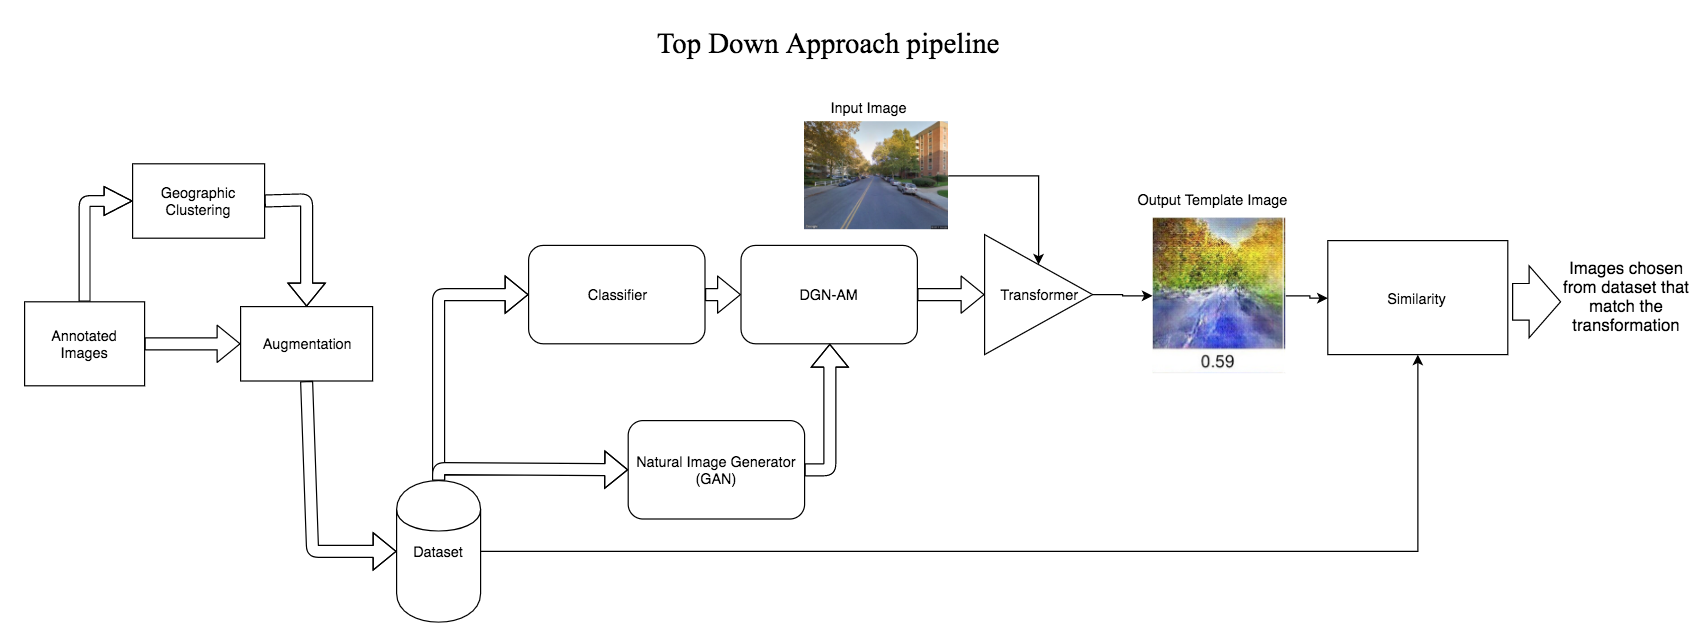
\includegraphics[width=1.8\columnwidth]{Plot/ExplainabilityPipeline_abstract.png}
	\caption{Process pipeline for the "Top Down" approach for explainability}
    \label{fig:pipeline}
\end{figure*}

\subsection{Pre-Processing: Data Clustering and Augmentation}
We assume that the input to the framework is simply a crawl of geo-referenced images, annotated for an arbitrary use case. The data needs to be preprocessed in two separate ways: Data clustering and Data Augmentation.
\subsubsection{Data Clustering}
%In the first step, we %need to 
%cluster data on the basis of some pre-determined attributes. %The clustering could be based on geographical context , visual similarity context or both. 
In urban images, the variance in structure and composition %between images 
can be extremely high. 
The main aim of data clustering is to reduce the diversity and variance in the image set. This is needed when working with  state of the art deep-learning classifiers, which generally work on highly specific classes of objects with low variance in the image semantics. Two clustering methods are listed below.
\begin{itemize}
	\item The most simple yet effective way to cluster data %could be 
	is based on geographical context. This can be done simply by using geographical boundaries of areas of interest and clustering images based on attributes like rural, urban, suburban, city etc.  This seems like an intuitive pre-processing step, as images from countryside look widely different compared to the images from the urban environment, and might be look visually diverse despite having similar annotations.
	\item %
	The other solution is to cluster images based on some visual/latent similarity measure. One possible way to do this is by extracting higher dimensional features, and clustering images based on these features.
\end{itemize} 

 
\subsubsection{Data Augmentation}
In the due process of clustering, it is expected that the total size of data available to train would reduce. Smaller data size implies that a machine learning model has a risk of over-fitting and in the worst case not learning anything at all. Hence there is a need to augment this clustered data with some additional real and transformed data. Some of the techniques that may be used are listed below.
\begin{itemize}
	\item The most common augmentation technique in deep learning literature is to do transformations on the image. Transformations like flipping images, cropping, adding noise , shifting color histograms can increase the data points for training and at the same time reduce the risks of over fitting.
	\item Because the images are geo tagged, one can augment the data by acquiring additional images which fall very close geographically to the original image. In this approach, care must be taken to maintain visual similarity of additional images. This can be achieved by several ways including, but not limited to, using higher dimensional features extracted using some pre-trained image models, to measure visual similarity (as described in the clustering section).
\end{itemize}. 

%\subsection{Classifier}

% In our case, we choose the classifier to be binary in nature because of the ranking distribution as seen in Fig \ref{fig:trueskill}. It is worth noting that the classification performance of this classifier would govern how articulately can you explain the network.

\subsection{Template Generator}
\par 
We now want to design a framework to transform any image $I$ into a template image $\hat{I_j}$ (as shown in Figure \ref{fig:pipeline}) %which is a synthetically perturbed version of $I$ such that it maximizes the activation for annotation class $y_j$. 
$\hat{I_j}$  is  a synthetic version of the original image, with added features and motifs that maximize class $y_j$. %The final step would transform this template image, into a natural image.
To produce the template image $\hat{I_j}$, we need the following components in place, 1) A classifier which learns how to distinguish between different image categories $y_i$ 2)  A generative model (GAN), that can generate samples from the distribution of the dataset images. 3) An activation maximization framework, that, based on the GAN generator, generates images that maximizes activation for a given annotation class \cite{dosovitskiy2016inverting} (our template images). 
\begin{itemize}
	\item{\textit{Classifier}}. %In order to produce template images, 
	To create synthetic representations of annotation classes, we first train a deep learning based classifier, that, given an image $I$, can correctly classify it in one of the $k$ classes. The aim of the rest of this pipeline is to explain \textit{what} the classifier is learning about the annotations. The assumption here is, once the classifier learns to discriminate amongst the classes, it also learns discriminative properties about the images that fall in those annotation categories. %Several works have shown that as a convolutional network trains, several semantic and object detectors emerge at higher abstraction levels in the network architecture. 
	\item \textit{Generator}. We train a generative adversarial network (GAN) which can generate an approximate natural looking image drawn from distribution of a particular class of images, similar to the one  in \cite{dosovitskiy2016inverting}. This GAN generator would learn to generate a natural-like image that represents the overall structure and knowledge about the Dataset.
	\item \textit{Activation Maximization}. We plug in the GAN and the classifier network into an Activation Maximisation (AM) framework. Given these components, an input image $I$, and a target class $y_i$, the AM transforms $I$ in an ideal image $\hat{I_j}$ ( that maximizes the activation for  class $y_i$). %The output of this step would be an image, which is very close to a natural image that the classifier is trained on, but has all the right motifs that maximizes the annotation class. 
	Essentially $\hat{I_j}$  is a representation of the overall knowledge about a particular annotation class, that the classifier network has learned through training. 
\end{itemize}	


\subsection{Similarity and inference}
In this final step we find a target image $I'$ from the dataset that is closely aligned, in terms of some visual similarity metric $E(I_1, I_2)$, with the generated template image  $\hat{I_j}$ . The result of this exercise is to find the most similar looking image to an input image $I$ that maximizes a particular annotation class $y_j$.% So in a sense we are transforming one natural image into another natural image so as to maximize some annotation class. 
The visual differences in these two natural images, can act as the subject of reasoning for the explainability.